% Prüfungsrelevant?
\documentclass[asp2.tex]{subfiles}
\begin{document}

\section{Aufbau SAP System}

\subsection{Aus Sicht des Vertriebs}

\begin{figure}[H]
    \begin{center}
        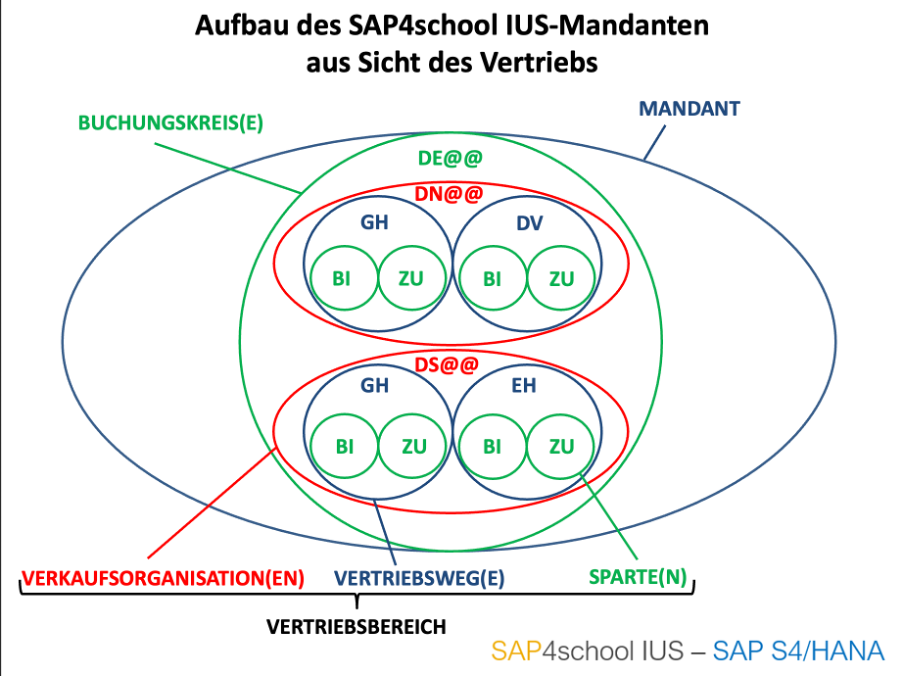
\includegraphics[width=1\textwidth]{SAP_Aufbau_Vertrieb.png}
    \end{center}
    \caption{ERP System aus Sicht des Vertriebs}
\end{figure}

\subsection{Aus Sicht der Produktion/Logistik}

\begin{figure}[H]
    \begin{center}
        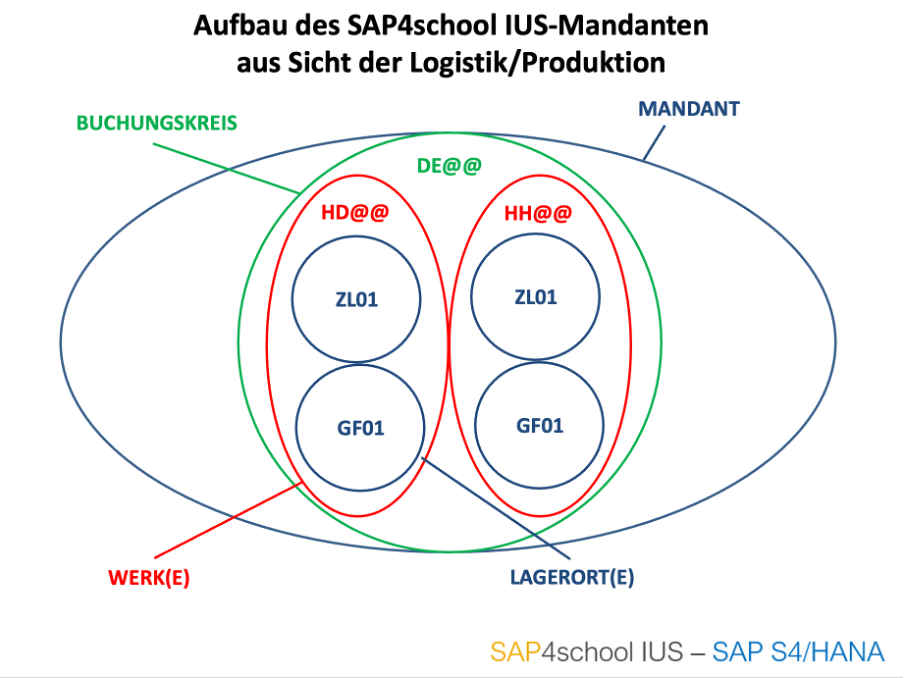
\includegraphics[width=1\textwidth]{SAP_Aufbau_Produktion.png}
    \end{center}
    \caption{ERP System aus Sicht der Produktion/Logistik}
\end{figure}

\subsection{Begriffe}

\subsubsection{ERP}

ERP (Enterprise Resource Planning), Unternehmensressourcenplanung. 
Es handelt sich dabei um eine Software, die Unternehmen dabei unterstützt, 
ihre Ressourcen effizienter zu planen, zu koordinieren und zu steuern. 
Die Hauptziele von ERP-Systemen sind die Optimierung von Geschäftsprozessen, 
die Reduzierung von Kosten und die Steigerung der Effizienz.

\subsubsection{Mandant}

\begin{outline}
    \1 Höchste Hierarchieebene eines SAP ERP-Systems.
    \1 Eine für sich handelsrechtlich, organisatorisch und datentechnisch abgeschlossene Einheit in einem SAP-System. 
\end{outline}

\subsubsection{Buchungskreise}

\begin{outline}
    \1 Ein Buchungskreis ist eine organisatorische Einheit in SAP, die für 
    die Buchhaltung zuständig ist. 
    \1 Jeder Buchungskreis erstellt seine eigenen Finanzberichte und ist 
    unabhängig von anderen Buchungskreisen.
\end{outline}

\subsubsection{Verkaufsorganisationen}

\begin{outline}
    \1 Eine Verkaufsorganisation ist eine Einheit in SAP, die sich auf den Vertrieb und Verkauf von Produkten konzentriert. 
    \1 Jede Verkaufsorganisation kann ihre eigenen Vertriebsstrukturen und -prozesse haben.
\end{outline}

\subsubsection{Werke}

\begin{outline}
    \1 Ein Werk repräsentiert in SAP einen physischen Ort, an dem Produkte hergestellt oder gelagert werden. 
    \1 Es ist mit der Produktions- und Lagerverwaltung verbunden.
\end{outline}

\subsubsection{Lagerorte}

\begin{outline}
    \1 Ein Lagerort ist ein definierter Ort, an dem Materialien oder Waren physisch gelagert werden. 
    \1 Innerhalb eines Werks können verschiedene Lagerorte existieren, um die Bestände effizient zu organisieren.
\end{outline}

\subsubsection{Sparten}

\begin{outline}
    \1 Eine Sparte ist eine organisatorische Einheit in SAP, die sich auf 
    bestimmte Geschäftsbereiche oder Produktlinien konzentriert. 
    \1 Es hilft, Geschäftsprozesse nach spezifischen Kriterien zu organisieren.
\end{outline}

\subsubsection{Vertriebsbereich}

Der Vertriebsbereich ist die Kombination von Verkaufsorganisation, Vertriebsweg und Sparte

subsection{Stammdaten}

Beispielsweise Kreditore, Debitoren, Material etc.

Sie werden unterteilt in:

\begin{outline}
    \1 Allgemeine Daten (Unternehmensweit)
    \1 Buchhaltungsdatem (Unterschiedlich je nach Buchungskreis)
    \1 Vertriebsbereichsdaten (Unterschiedlich je nach Vertriebsbereich)
        \1 z.B. Preis eines Fahrrades ist unterschiedlich für Großhandel und Einzelhandel
        \1 Zahlungsbedingungen
        \1 Lieferbedingungen je Kunde unterschiedlich
\end{outline}

\section{Industrie 4.0}

Industrie 4.0 ist ein Konzept der intelligenten Vernetzung von Produktionsprozessen, 
bei dem fortschrittliche Technologien wie das Internet der Dinge (IoT), 
künstliche Intelligenz (KI) und Big Data eingesetzt werden. 
Ziel ist die Schaffung hochflexibler und effizienter Fertigungssysteme, 
die autonom agieren können, sich selbst optimieren und nahtlos mit anderen 
Systemen kommunizieren. Dieses Konzept zielt darauf ab, die Industrie in eine 
Ära der digitalen Transformation zu führen, die durch Integration, Automatisierung 
und datenbasierte Entscheidungsfindung gekennzeichnet ist.

\subsection{Begriffe}

\subsubsection{Cyber-physisches System (CPS)}

Systeme, die die mechanischen und elektronischen Teile der Fabrik 
um softwaretechnische Komponenten er-gänzen und miteinander verbinden. 
Der Datentransfer sowie die Kontrolle bzw. Steuerung erfolgen über eine 
Infrastruktur wie das Internet in Echtzeit 

\subsubsection{Mass customization}

Strategischer Trend, der die Vorteile der Massenproduktion mit dem Wunsch 
der Kunden nach Individualisierung vereinbart. 
Beispiele im Turnschuhmarkt sind  „mi adidas“ oder „NikeID“.  

\subsubsection{MES}

Direkte Anbindung an die verteilten Systeme der Prozessautomatisierung und 
ermöglicht die Führung, Lenkung, Steuerung oder Kontrolle der Produktion in Echtzeit.

\section{SAP Notes für Arbeiten}

\begin{outline}
    \1 In der Arbeit darf das Blatt "Vorlage Organisationsdaten S4 HANA" benutzt werden.
    \1 Alles findet hier statt: Stammdaten -> Verkauf -> Debitorenstamm -> anzeigen
    \1 Bei der Suche nach einem Debitor ist der Nachname der Firmenname.
        \1 * ist eine Wildcard (*SAP* wäre alles, das SAP irgendwo im Namen hat)
        \1 Bei der Suche MUSS "*<SAP-Kennnummer>" als Geschäftspartner angegeben werden (Bei mir *023)
            \1 Die Kennnummer ist auf dem Hilfsblatt oben zu finden
\end{outline}

\end{document}